\chapter{프리드만 동역학: 물질, 복사, 진공 에너지}

\lectureoverview{팽창하는 우주의 운동학은 한 줄로 표현할 수 있다. 물리적 거리 간격은 척도인자 \(a(t)\)에 따라 커진다. 이제 문제는 이 함수가 어떤 것인지 결정하는 것이다. 뉴턴 역학의 에너지 보존으로부터 평탄한 공간의 프리드만 방정식을 다시 유도하고, 먼저 보통 물질의 경우를 풀어 본 뒤 복사와 진공 에너지가 왜 전혀 다른 우주 역사를 낳는지 살펴보겠다.}

\section{설명해야 할 기하}

고정된 우주 시각에 보면 우주는 큰 규모에서 균질하고 등방적으로 보인다. 은하와 은하단, 초은하단은 분명 실제 구조이지만, 수억 또는 수십억 광년 규모로 보면 그 분포는 놀라울 만큼 균일해진다. 이러한 경험적 규칙성을 우주론적 원리라고 한다. 이름이 붙었다고 해서 정리가 되는 것은 아니다. 이 원리의 근거는 관측에 있다.

두 번째 경험적 사실도 있다. 현재의 정확도 안에서 보면 큰 공간 삼각형은 유클리드 삼각형처럼 거동한다. 축구장을 측량하는 예를 떠올리면 이해하기 쉽다. 팽팽하게 당긴 선으로 만든 삼각형의 내각의 합이 \(180^\circ\)이라 해도, 지구 전체가 평평하다는 것이 증명되지는 않는다. 지구의 곡률 반지름이 경기장에 비해 크다는 뜻이다. 우주를 측량할 때도 논리는 같다. 공간의 곡률 반지름은 매우 클 수 있지만, 관측 가능한 영역에서는 평탄하다고 근사할 수 있다.

기준이 되는 기하학은 민코프스키 시공간이다. \begin{equation}
  d\tau^2=dt^2-\left(dx^2+dy^2+dz^2\right).
  \label{eq:l09-minkowski}
\end{equation}대괄호 안은 단순히 3차원 유클리드 거리 요소다. 이와 달리 일반 상대성 이론에서 좌표 미분의 계수는 장이다. 이 계수들은 위치와 시간에 따라 달라질 수 있으며, 혼합항이 나타날 수도 있다. 이러한 계량 계수는 뉴턴 중력장의 상대론적 후계자다.

\begin{figure}[H]\centering
  \includegraphics[width=0.72\textwidth]{lecture_09_figure_01.png}\caption{강의 첫머리에 적은 민코프스키 고유시간 요소. 출처 프레임 00:01:50.}\label{fig:l09-minkowski-board}\end{figure}

공간적으로 평탄한 팽창 우주에서는 균질성과 등방성 때문에 시간에 따라 변하는 척도인자 하나만 남는다. \begin{equation}
  d\tau^2=dt^2-a^2(t)\left(dx^2+dy^2+dz^2\right).
  \label{eq:l09-flat-frw}
\end{equation}\(c=1\)인 단위를 사용하므로 시간과 길이는 같은 차원을 갖는다. 일관된 관례는 두 가지다. \(x,y,z\)에 길이 차원을 부여하고 \(a\)을 무차원으로 둘 수도 있고, \(x,y,z\)을 무차원 표지로 취급하고 \(a\)에 길이 차원을 부여할 수도 있다. 강의에서는 \(a(t)\)의 물리적 의미가 분명히 드러나는 두 번째 관례를 사용한다.

\begin{figure}[H]\centering
  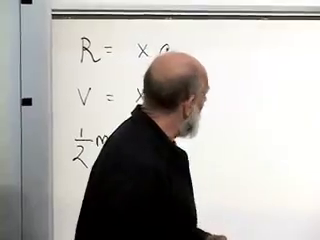
\includegraphics[width=0.72\textwidth]{lecture_09_figure_02.png}\caption{유클리드 공간 선요소에 척도인자가 곱해진 평탄 팽창 계량. 출처 프레임 00:09:12.}\label{fig:l09-expanding-metric-board}\end{figure}

고무판 위에 좌표를 그려 놓았다고 상상해 보자. 좌표 표지는 판에 붙어 그대로 있지만, 표지 사이의 물리적 거리는 커진다. 따라서 “\(x=0\)에서 \(x=1\)까지”와 같은 좌표 차이는 표지 두 개를 가리킬 뿐이다. 그 간격이 나타내는 거리는 \(a(t)\)이다. 이 척도인자를 지배하는 방정식을 찾는 것이 이번 강의의 동역학 문제다.

\section{닫힌 공간, 평탄한 공간, 열린 공간의 기하}

평탄성은 관측상의 단순화이지 균질성의 귀결은 아니다. 균질하고 등방적인 공간 기하는 곡률이 양수, 0, 음수인 세 가지다. 양의 곡률인 경우를 이해하려면 차원을 정확히 구분하는 것이 도움이 된다.

\begin{equation}
  X_1^2+X_2^2=R^2
\end{equation}의 자취는 원, 즉 일구 \(S^1\)다. 그 안을 채운 영역은 원판이며 이차원 공이라고도 한다. 매장 좌표를 하나 더하면 \begin{equation}
  X_1^2+X_2^2+X_3^2=R^2,
\end{equation}이 되고, 이는 보통의 이구 \(S^2\)다. 매장 좌표를 하나 더 추가하면 \begin{equation}
  X_1^2+X_2^2+X_3^2+X_4^2=R^2,
  \label{eq:l09-three-sphere}
\end{equation}이 되며, 이는 그 자체로 삼차원 공간인 삼구 \(S^3\)다. 우리는 그것이 매장된 4차원 공간을 그려 볼 수 없지만, 내재적 기하가 존재하는 데 그 매장은 필요하지 않다.

\begin{figure}[H]\centering
  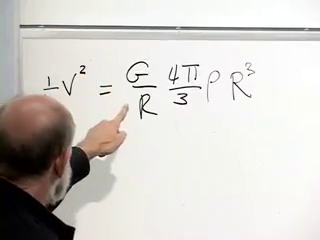
\includegraphics[width=0.72\textwidth]{lecture_09_figure_03.png}\caption{삼구를 소개할 때 사용한 매장 방정식. 출처 프레임 00:16:40.}\label{fig:l09-three-sphere-board}\end{figure}

이상적인 구의 모든 점은 기하학적으로 서로 동등하고, 한 점에서 모든 방향도 서로 동등하다. 따라서 구는 균질하면서 등방적이다. 반지름에 \(a(t)\)를 곱하면 구면 위에서 특정한 중심을 정하지 않고 공간 전체가 팽창하거나 수축한다. 이런 우주의 과거를 거슬러 올라가도 모든 물질이 외부의 빈 공간에 있는 한 특별한 지점에 모이는 것은 아니다. 공간 전체가 작아지므로 모든 점 쌍의 거리가 가까워진다. 빅뱅은 공간의 한 점에서 일어난 폭발이 아니다.

양의 곡률을 가진 구면에서 측지 삼각형의 내각의 합은 \(180^\circ\)보다 크다. 평탄한 삼각형의 내각의 합은 정확히 \(180^\circ\)이다. 안장으로 불완전하게 나타낼 수 있는 균질한 음의 곡률 기하에서는 내각의 합이 \(180^\circ\)보다 작다. 이러한 내재적 검사를 통해 세 경우를 구별할 수 있다.

\begin{figure}[H]\centering
  \includegraphics[width=0.72\textwidth]{lecture_09_figure_07.png}\caption{삼각형의 특징적인 모양으로 나타낸 양의 곡률, 영 곡률, 음의 곡률. 출처 프레임 00:37:30.}\label{fig:l09-curvature-board}\end{figure}

국소 계량이 완벽하게 평탄하다는 사실만으로 공간의 위상적 구조가 무한하다고 증명되지는 않는다. 콤팩트한 평탄 위상도 수학적으로 가능하지만, 이 강의에서는 가장 단순한 무한 유클리드 모형을 채택한다. \editorialnote{이러한 전역 위상에 관한 단서는 이후의 국소 동역학에는 필요하지 않다.}

\section{공변 좌표와 허블 법칙}

이제 팽창하는 평탄한 판으로 돌아가 그 위에 좌표 격자를 그려 보자. 공변 좌표계에서 격자는 큰 규모의 물질 흐름을 따라 함께 팽창한다. 은하, 또는 더 정확히는 충분히 거칠게 평균한 은하단은 물리적으로 다른 공변 물체와의 거리가 변하더라도 좌표 표지는 대체로 그대로 유지한다.

\begin{figure}[H]\centering
  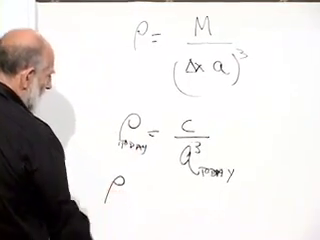
\includegraphics[width=0.72\textwidth]{lecture_09_figure_04.png}\caption{팽창하는 공간 판을 따라 움직이는 좌표 격자. 출처 프레임 00:22:20.}\label{fig:l09-comoving-grid-board}\end{figure}

\(x\)축을 따라 고정된 공변 간격 \(\Delta x\)만큼 떨어진 두 물체 사이의 물리적 거리는 다음과 같다. \begin{equation}
  D(t)=a(t)\,\Delta x.
  \label{eq:l09-physical-distance}
\end{equation}\(\Delta x\)을 고정한 채 미분하면 다음을 얻는다. \begin{equation}
  v(t)=\dot a(t)\,\Delta x
      =\frac{\dot a(t)}{a(t)}D(t).
\end{equation}다음과 같이 정의하면 \begin{equation}
  H(t)\equiv\frac{\dot a(t)}{a(t)},
  \label{eq:l09-hubble-parameter}
\end{equation}허블 법칙을 얻는다. \begin{equation}
  v=H(t)D.
  \label{eq:l09-hubble-law}
\end{equation}“허블 상수”에서 “상수”라는 말은 정해진 우주 시각에 공간 전체에서 일정하다는 뜻이다. 우주의 역사 전체에 걸쳐 일정하다는 뜻은 아니다.

\begin{figure}[H]\centering
  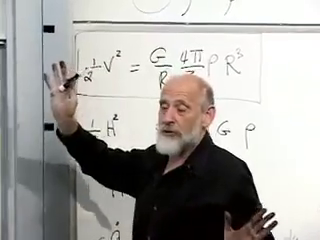
\includegraphics[width=0.72\textwidth]{lecture_09_figure_05.png}\caption{칠판 유도 \(D=a\Delta x\), \(v=(\dot a/a)D=HD\). 출처 프레임 00:26:40.}\label{fig:l09-hubble-board}\end{figure}

\begin{classroomqa}\audiencequestion{먼 은하를 더 이른 시기의 모습으로 관측했다면, 그곳에서 추론한 허블 매개변수도 오늘날 가까운 곳에서 측정한 값과 정말 같아야 할까요?}\lecturerresponse{되돌아보는 시간이 우주의 나이에 비해 짧을 때만 그렇습니다. 적당한 거리에서는 \(H(t)\)가 거의 변하지 않으므로 하나의 값으로 나타내도 충분합니다. 진정한 우주론적 거리를 관측할 때는 더 이른 시기의 우주를 보는 것이므로 \(a\)와 \(H\)의 시간 변화를 고려해야 합니다. 이것이 척도인자의 동역학 방정식이 필요한 이유 중 하나입니다.}\end{classroomqa}

\section{팽창 좌표계에서의 영광선}

\begin{classroomqa}\audiencequestion{척도인자는 먼 은하 사이를 전파하는 빛에도 영향을 줄까요?}\lecturerresponse{빛은 영 궤적을 따르므로 \(d\tau=0\)이다. 양의 \(x\)축을 따라 움직이는 광선에서는 \(dy=dz=0\)이고, 팽창 계량은 다음을 준다. \begin{align}
  0&=dt^2-a^2(t)dx^2,
  &dt&=a(t)dx,\notag\\
  &&\frac{dx}{dt}&=\frac{1}{a(t)}.
  \label{eq:l09-null-ray}
\end{align}\(a(t)\)가 커질수록 좌표 속도는 작아지지만, 국소적으로 측정하는 빛의 물리적 속도는 여전히 \(c=1\)이다. 고정된 좌표 간격이 나타내는 물리적 거리는 점점 커진다.}\end{classroomqa}

\begin{figure}[H]\centering
  \includegraphics[width=0.72\textwidth]{lecture_09_figure_06.png}\caption{방사형 빛 전파의 영 조건과 \(dt=a(t)dx\). 출처 프레임 00:30:54.}\label{fig:l09-null-board}\end{figure}

좌표를 선택하면 같은 사실을 “멀리 갈수록 빛이 느려진다”라고 표현할 수도 있지만, 그러면 길이와 시계에 대한 설명이 그에 따라 다루기 까다로워진다. 팽창하는 공간이라는 표현이 더 간결한 이유는 모든 자유낙하 관측자가 같은 빛의 속도를 측정한다는 국소적 진술을 그대로 보존하기 때문이다.

\begin{classroomqa}\audiencequestion{}먼 은하에서도 국소적인 빛의 전파와 원자 물리가 같다는 증거가 있나요?\lecturerresponse{무차원 비교만이 조작적으로 의미가 있다. 원자 크기를 길이의 단위로, 원자 또는 핵의 주기를 시간의 단위로 정한 다음, 빛이 그 길이를 가로지르는 데 그러한 주기가 몇 번 필요한지 물어보면 된다. 스펙트럼 관측은 이런 무차원비가 먼 영역에서도 같다는 진술을 뒷받침한다. 증거는 간접적이지만, 국소 법칙의 균일성을 검증하는 방법이 바로 이런 비교다.}\end{classroomqa}

관측 가능한 우주가 극도로 작았을 때는 그에 맞는 광행 시간 단위로 보면 빛이 일정한 물리적 영역을 빠르게 가로지를 수 있었다. 그렇다고 \(c\)가 달랐다는 뜻은 아니다. 영역 자체가 작았다는 뜻이다.

\section{우주 안의 뉴턴 구}

이제 운동학에서 동역학으로 넘어가자. 우리가 원점에 있다고 놓고, 많은 은하와 은하단을 포함할 만큼 큰 구를 그린다. 그 경계에 있는 은하 하나를 택한다. 균질한 우주에서는 질량 분포가 우리를 중심으로 구대칭이므로, 뉴턴의 껍질 정리에 따라 다음 두 가지 중요한 사실이 성립한다. \begin{enumerate}\item 선택한 반지름 바깥에 구형으로 분포한 모든 물질은 경계 은하에 순 뉴턴 힘을 전혀 가하지 않는다. \item 구 안에 있는 모든 물질은 이 방사 방향 운동에 대해 중심에 모여 있는 것처럼 작용한다. \end{enumerate}우리가 정지해 있는 기준계를 사용하므로, 다음 논증에서 속도와 가속도는 우리에 대한 값으로 측정한다.

\begin{figure}[H]\centering
  \includegraphics[width=0.72\textwidth]{lecture_09_figure_08.png}\caption{껍질 정리의 구성: 중심에 있는 우리와 균질한 큰 구의 경계에 놓인 시험 은하. 출처 프레임 00:41:10.}\label{fig:l09-shell-board}\end{figure}

\begin{figure}[H]\centering
  \begin{tikzpicture}[scale=0.92,>=Latex]
    \draw[thick] (0,0) circle (2.35);
    \fill (0,0) circle (2pt) node[below left] {us};
    \fill (2.35,0) circle (2.2pt) node[right] {test galaxy \(m\)};
    \draw[->,thick,blue!65!black] (0.18,0) -- (2.15,0)
      node[midway,above] {\(R=a(t)x\)};
    \draw[->,thick,red!65!black] (2.35,0.12) -- (3.25,0.12)
      node[midway,above] {\(v=\dot a(t)x\)};
    \node[align=center,text width=7cm] at (0,-2.85)
      {outside shells cancel;\\enclosed mass acts at the center};
  \end{tikzpicture}\caption{뉴턴 역학의 구성을 깔끔하게 다시 그린 그림.}\label{fig:l09-shell-clean}\end{figure}

은하의 공변 좌표 \(x\)가 고정되어 있다면, 물리적 반지름과 속도는 다음과 같다. \begin{equation}
  R(t)=x a(t),
  \qquad
  v(t)=x\dot a(t)=H(t)R(t).
  \label{eq:l09-radius-velocity}
\end{equation}구 안에 포함된 질량을 \(M\), 시험 은하의 질량을 \(m\)라 하자. 뉴턴 역학에서 에너지는 다음과 같다. \begin{equation}
  E=\frac12 m v^2-\frac{GMm}{R}.
  \label{eq:l09-newtonian-energy}
\end{equation}

\begin{figure}[H]\centering
  \includegraphics[width=0.72\textwidth]{lecture_09_figure_09.png}\caption{칠판의 전체 전개 \(R=xa\), \(v=x\dot a\) 및 \(E=0\)에 특화한 뉴턴 에너지 방정식. 출처 프레임 00:48:40.}\label{fig:l09-energy-board}\end{figure}

에너지는 양수, 0, 음수일 수 있다. 탈출과 재붕괴의 경계인 \(E=0\)인 경우부터 살펴보자. 이때는 다음과 같다. \begin{equation}
  \frac12 v^2=\frac{GM}{R}.
  \label{eq:l09-zero-energy}
\end{equation}

\begin{classroomqa}\audiencequestion{은 전체 에너지가 0이라는 것은 멀어지는 은하에 대해 어떤 뜻인가요?}\lecturerresponse{정확히 탈출 속도에 해당하는 경우다. 양의 에너지는 탈출 속도보다 빠른 운동을 뜻하고, 음의 에너지는 탈출 속도보다 느린 운동을 뜻하며, 물질만 있는 뉴턴 역학의 그림에서는 결국 되돌아온다. 우리는 이 두 가능성 사이의 경계에서 출발해 평탄 방정식을 유도한 다음 다른 부호의 경우를 살펴보겠다.}\end{classroomqa}

\begin{classroomqa}\audiencequestion{\(M\)구 안에 포함된 질량 }은 구가 팽창할 때 변하나요?\lecturerresponse{아니다. 구는 공변하므로 같은 입자들이 계속 그 안에 머문다. 물리적 부피는 커지고 밀도는 낮아지지만, 구 안에 포함된 전체 질량은 일정하게 유지된다. \(M\)과 \(\rho(t)\)의 차이를 구별하는 것이 중요하다.}\end{classroomqa}

균질한 밀도 \(\rho(t)\)에 대해 다음이 성립한다. \begin{equation}
  M=\frac{4\pi}{3}\rho(t)R^3.
  \label{eq:l09-enclosed-mass}
\end{equation}이를 \eqref{eq:l09-zero-energy}에 대입하면 다음을 얻는다. \begin{equation}
  \frac12 v^2
  =\frac{G}{R}\left(\frac{4\pi}{3}\rho R^3\right).
  \label{eq:l09-enclosed-energy}
\end{equation}

\begin{figure}[H]\centering
  \includegraphics[width=0.72\textwidth]{lecture_09_figure_10.png}\caption{영 에너지 방정식에 구 안의 질량을 대입한 모습. 출처 프레임 00:54:16.060.}\label{fig:l09-enclosed-mass-board}\end{figure}

\(v=HR\)를 사용하면 다음을 얻는다. \begin{align}
  \frac12 H^2R^2
    &=\frac{4\pi G}{3}\rho R^2,\\
  H^2
    &=\frac{8\pi G}{3}\rho.
\end{align}따라서 영 에너지, 공간 평탄 팽창 법칙은 다음과 같다. \begin{equation}
  \boxed{\left(\frac{\dot a}{a}\right)^2
  =\frac{8\pi G}{3}\rho(t)}.
  \label{eq:l09-flat-friedmann}
\end{equation}\(R^2\)의 소거는 우연이 아니다. 균질한 우주에서는 시험 물체로 어떤 공변 은하를 택하더라도 \(H(t)\)가 같아야 한다.

\begin{figure}[H]\centering
  \includegraphics[width=0.72\textwidth]{lecture_09_figure_11.png}\caption{칠판에 나타낸 반지름의 소거와 그 결과인 평탄 프리드만 관계식. 출처 프레임 00:57:30.}\label{fig:l09-friedmann-board}\end{figure}

\begin{classroomqa}
\audiencequestion{영에너지 관계를 뒷받침하는 증거가 있나요?}
\lecturerresponse{양변은 모두 관측을 통해 추론할 수 있습니다. \(H\)는 후퇴 자료에서, \(\rho\)는 별과 기체, 암흑 물질, 진공 에너지를 모두 고려해 구할 수 있습니다. 강의 당시의 비교에서는 두 양이 퍼센트 수준의 정확도로 일치하는 것으로 나타났습니다. 다만 중요한 조건이 있습니다. 모든 형태의 에너지를 포함해야 하며, 이후의 진공 에너지 논의에 따르면 단순한 탈출 속도 해석은 달라집니다.}
\end{classroomqa}

\(c=1\)인 단위계에서는 질량 밀도와 에너지 밀도의 단위가 같다. 따라서 기호 \(\rho\)는 논의 중인 성분에 해당하는 전체 에너지 밀도를 나타낸다.

\section{일반 물질과 2/3 법칙}

\eqref{eq:l09-flat-friedmann}만으로는 아직 방정식이 완결되지 않는다. \(\rho(t)\)가 어떻게 변하는지 알아야 한다. 먼저 천천히 움직이는 비상대론적 입자들로 공변 직육면체를 채워 보자. 상자의 좌표상 변 길이는 고정되어 있지만, 물리적 부피는 다음과 같이 커진다. \begin{equation}
  V(t)=a^3(t)\,\Delta x\,\Delta y\,\Delta z.
\end{equation}상자 안의 입자 수와 정지 질량은 그대로이므로 다음과 같다. \begin{equation}
  \rho_{\mathrm m}(t)=\frac{C_{\mathrm m}}{a^3(t)}.
  \label{eq:l09-matter-dilution}
\end{equation}현재 시각 \(t_0\)을 기준으로 정규화하면 다음과 같다. \begin{equation}
  \frac{\rho_{\mathrm m}(t)}{\rho_{\mathrm m,0}}
  =\left(\frac{a_0}{a(t)}\right)^3.
  \label{eq:l09-matter-normalized}
\end{equation}

\begin{figure}[H]\centering
  \includegraphics[width=0.72\textwidth]{lecture_09_figure_12.png}\caption{물질 밀도, 그 \(a^{-3}\) 희석, 현재 시점의 정규화. 출처 프레임 01:04:47.940.}\label{fig:l09-density-board}\end{figure}

\begin{classroomqa}\audiencequestion{}현재 우주의 대략적인 에너지 밀도는 얼마이며, 보통 원자만으로 이를 설명할 수 있나요?\lecturerresponse{눈에 보이는 중입자 물질만 세어서는 답의 일부만 얻는다. 암흑 물질과 암흑 에너지도 질량과 에너지의 등가물로 포함해야 한다. 강의에서는 정밀한 목록보다 규모를 강조하며, 에너지 밀도의 대략적인 범위를 수소 원자 질량으로 환산한 입자 하나에서 수십 개 정도의 세제곱미터당 값으로 제시한다.}\end{classroomqa}

\eqref{eq:l09-matter-dilution}를 \eqref{eq:l09-flat-friedmann}에 대입하고 시간에 무관한 인자들을 모두 양의 상수 \(C\)에 포함시키면 다음을 얻는다. \begin{equation}
  \left(\frac{\dot a}{a}\right)^2=\frac{C}{a^3},
  \qquad
  \dot a^2=\frac{C}{a}.
  \label{eq:l09-matter-ode}
\end{equation}방정식을 푸는 방법은 명료하게 두 가지다. 멱법칙 해 \(a=K t^p\)를 가정하면 다음 조건이 필요하다. \begin{equation}
  p-1=-\frac{p}{2},
  \qquad p=\frac23.
\end{equation}같은 방정식에서 팽창에 해당하는 제곱근 가지를 택해 적분할 수도 있다. \begin{equation}
  a^{1/2}\frac{da}{dt}=\sqrt C,
  \qquad
  \int a^{1/2}da=\sqrt C\int dt,
\end{equation}따라서 빅뱅을 시간의 원점으로 택하면 다음과 같다. \begin{equation}
  a^{3/2}\propto t,
  \qquad
  \boxed{a(t)\propto t^{2/3}}.
  \label{eq:l09-matter-solution}
\end{equation}실시간 칠판 유도에서는 계수를 맞추는 과정에서 인자 하나가 잠시 빠졌지만, 적분으로 돌아가 지수를 확인했다. 이 노트에는 그 확인 과정을 유지하되, 수정된 대수식만 제시한다.

\begin{figure}[H]\centering
  \includegraphics[width=0.72\textwidth]{lecture_09_figure_13.png}\caption{멱법칙 가정과 상자 안에 표시한 지수 \(p=2/3\). 출처 프레임 01:13:05.}\label{fig:l09-matter-solution-board}\end{figure}

해를 미분하면 다음을 얻는다. \begin{equation}
  H(t)=\frac{\dot a}{a}=\frac{2}{3t}.
  \label{eq:l09-matter-hubble}
\end{equation}과거에는 허블 매개변수가 더 컸다. 따라서 되돌아보는 시간이 상당히 길 정도로 먼 곳을 볼 때는 오늘날의 \(H_0\)를 그대로 써서 국소적 선형 관계를 연장해서는 안 된다.

\begin{figure}[H]\centering
  \includegraphics[width=0.72\textwidth]{lecture_09_figure_14.png}\caption{\(\dot a/a\)에 \(a\propto t^{2/3}\)를 대입하면 다음을 얻는다. \(H=2/(3t)\). 출처 프레임 01:20:42.}\label{fig:l09-hubble-time-board}\end{figure}

\section{에너지 부호와 공간 곡률}

뉴턴 역학의 논증으로 영 에너지인 평탄한 경우까지 유도했다. 일반 상대성 이론에는 껍질 정리만으로는 얻을 수 없는 사실이 하나 더 있다. 뉴턴식 비에너지의 부호는 공간 곡률의 부호에 대응한다.
\begin{center}\begin{tabular}{@{}>{\raggedright\arraybackslash}p{0.20\linewidth}
                    >{\raggedright\arraybackslash}p{0.29\linewidth}
                    >{\raggedright\arraybackslash}p{0.37\linewidth}@{}}\toprule
  전체 에너지&공간 곡률&물질만 있을 때의 운명\\
\midrule
  양수&음수(열린 우주)&영원히 팽창\\
0&0(평탄한 우주)&탈출 경계에 가까워진다\\
음수&양수(닫힌 우주)&팽창하다가 방향을 바꾸어 재붕괴한다\\
\bottomrule
\end{tabular}\end{center}마지막 열은 진공 에너지가 없다고 가정한다. 발사체의 비유에서 양의 에너지는 탈출 속도보다 빠른 경우, 0은 정확히 탈출 속도인 경우, 음의 에너지는 탈출 속도보다 느린 경우를 뜻한다. 아인슈타인 방정식은 이 세 경우를 각각 열린 공간, 평탄한 공간, 닫힌 공간 기하와 연결한다.

\section{광자와 1/2 법칙}

물질 법칙 \(\rho\propto a^{-3}\)은 입자 수밀도가 낮아지는 동안 각 입자의 에너지는 대략 일정하다고 가정한다. 광자는 이 가정을 따르지 않는다. 광자의 경우 \begin{equation}
  E=h\nu=\frac{hc}{\lambda}.
\end{equation}팽창하면 파장이 척도인자에 비례해 늘어난다. \begin{equation}
  \lambda\propto a,
  \qquad E\propto a^{-1}.
\end{equation}광자 수밀도는 여전히 \(a^{-3}\)에 따라 낮아지며, 각 광자의 에너지에도 \(a^{-1}\)라는 인자가 하나 더 들어간다. 따라서 다음과 같다. \begin{equation}
  \boxed{\rho_{\mathrm r}(t)\propto a^{-4}(t)}.
  \label{eq:l09-radiation-dilution}
\end{equation}

기타 줄의 비유는 물리적 상황을 잘 보여 준다. 줄을 튕긴 뒤 진동하는 부분을 길게 늘이면 파장이 늘고 음높이가 낮아진다. 팽창하는 공변 상자 안의 광자 모드도 비슷하게 거동한다. 이 상황을 거꾸로 보면 압축 시 파장이 짧아지고 광자 에너지가 커진다.

\begin{figure}[H]\centering
  \includegraphics[width=0.72\textwidth]{lecture_09_figure_15.png}\caption{칠판에서 물질 밀도 관계식을 복사 밀도 스케일링 \(\rho_{\mathrm r}\propto a^{-4}\)까지 확장한 모습. 출처 프레임 01:29:20.}\label{fig:l09-radiation-board}\end{figure}

\(\rho_{\mathrm r}\propto a^{-4}\)를 평탄 프리드만 방정식에 대입하면 다음과 같다. \begin{equation}
  \left(\frac{\dot a}{a}\right)^2=\frac{C_{\mathrm r}}{a^4},
  \qquad
  \dot a\propto a^{-1},
\end{equation}그러므로 다음을 얻는다. \begin{equation}
  \boxed{a(t)\propto t^{1/2}}.
  \label{eq:l09-radiation-solution}
\end{equation}이는 \(t^{2/3}\)보다 느리게 증가한다. 충분히 과거로 거슬러 올라가면 \(a^{-4}\)가 \(a\)가 감소할수록 \(a^{-3}\)보다 더 빠르게 커지므로 복사가 보통 물질보다 우세해진다. 강의에서는 척도인자가 오늘날보다 대략 천 배 작았던 시기를 물질과 복사의 교차 시점으로 잡는다. 그보다 앞선 우주는 복사가 지배했고, 그 이후에는 오랜 기간 물질이 지배했다.

\section{진공 에너지와 지수 팽창}

진공 에너지는 정반대의 스케일링 거동을 보인다. 진공 에너지의 밀도는 빈 공간의 성질이므로 우주가 팽창해도 희석되지 않는다. \begin{equation}
  \rho_\Lambda=\text{constant}.
  \label{eq:l09-vacuum-density}
\end{equation}보통 물질과 복사는 과거로 갈수록 밀도가 높아지지만, 이 항은 그렇지 않다. 따라서 초기 우주에서는 영향이 작았고, 다른 성분들이 희석됨에 따라 점점 중요해진다. 강의에서는 당시 추정치에 따라 진공 에너지가 오늘날 우주 에너지 밀도의 약 \(70\%\)를 차지한다고 본다.

\(\rho_\Lambda\)가 일정하면 방정식 \eqref{eq:l09-flat-friedmann}에서 팽창률도 일정해진다. \begin{equation}
  H_\Lambda=\sqrt{\frac{8\pi G}{3}\rho_\Lambda},
  \qquad
  \frac{\dot a}{a}=H_\Lambda.
\end{equation}따라서 다음과 같다. \begin{equation}
  \boxed{a(t)=a(t_i)e^{H_\Lambda(t-t_i)}}.
  \label{eq:l09-vacuum-solution}
\end{equation}

\begin{figure}[H]\centering
  \includegraphics[width=0.72\textwidth]{lecture_09_figure_16.png}\caption{지수 팽창으로 이어지는 일정한 밀도 방정식. 출처 프레임 01:35:48.}\label{fig:l09-vacuum-board}\end{figure}

강의에서 언급한 관측 규모에서는 우주의 선형 크기가 대략 백억 년에서 백이십억 년에 걸쳐 두 배가 됩니다. 이 작지만 0이 아닌 진공 밀도의 기원은 여전히 설명되지 않았습니다. 그것의 존재와 팽창에 미치는 영향은 관측으로 확인된 사실입니다.

\begin{classroomqa}\audiencequestion{}이 논의에서 진공 에너지는 암흑 에너지와 같은 것인가요?\lecturerresponse{그렇다. 여기서 “암흑 에너지”는 일정한 진공 에너지 밀도, 즉 우주 상수를 뜻한다. 시간에 따라 변하는 더 일반적인 암흑 에너지 모형도 상정할 수 있지만, 이 강의의 계산에서는 다루지 않는다.}\end{classroomqa}

\section{팽창 우주가 빛을 적색편이시키는 방식}

\begin{classroomqa}\audiencequestion{우리가 팽창하는 공변 좌표를 택했다는 이유만으로 광자가 어떻게 그 사실을 알아차리고 에너지를 낮추나요?}\lecturerresponse{광자는 우리의 좌표 표지에 반응하지 않는다. 물리적 거리 간격이 변하는 기하를 따라 전파된다. 물리적 크기가 두 배가 되는 영역을 차지한 파동열은 파장도 두 배가 된다. 공변 좌표는 이러한 늘어남을 간결하게 기술할 뿐, 그 원인은 아니다.}\end{classroomqa}

\begin{classroomqa}\audiencequestion{오늘날 우리에게 도달하는 배경 광자는 어디에서 오는 건가요?}\lecturerresponse{더 먼 곳을 본다는 것은 더 이른 시기를 본다는 뜻이다. 더 거슬러 가면 우주의 물질이 이온화된 플라스마였던 시기를 보게 된다. 이때 광자는 자유 전하 입자에 반복해서 산란되어 우주가 불투명했다. 광자가 마지막으로 자유롭게 출발해 우리에게 올 수 있었던 경계는 관측자를 둘러싼 구면으로 보인다. 이것이 마지막 산란면이다.}\end{classroomqa}

\begin{figure}[H]\centering
  \includegraphics[width=0.72\textwidth]{lecture_09_figure_17.png}\caption{관측자를 중심으로 마지막 산란면과 점점 멀어지는 껍질을 그린 그림. 출처 프레임 01:42:05.}\label{fig:l09-last-scattering-board}\end{figure}

\begin{figure}[H]\centering
  \begin{tikzpicture}[scale=0.9,>=Latex]
    \fill (0,0) circle (2pt) node[below] {observer};
    \draw[thick,orange!70!black] (0,0) circle (2.55);
    \node[orange!70!black,align=center] at (0,3.05)
      {surface of last scattering};
    \foreach \a in {25,75,145,210,285,335}{
      \draw[->,blue!60!black] ({2.55*cos(\a)},{2.55*sin(\a)}) --
        ({1.7*cos(\a)},{1.7*sin(\a)});
    }
    \draw[decorate,decoration={snake,amplitude=1.5pt,segment length=7pt},
      red!65!black,thick,->] (-2.5,0) -- (-0.15,0);
    \node[red!65!black,below] at (-1.35,-0.15)
      {redshifted photon};
  \end{tikzpicture}\caption{마지막 산란 그림을 깔끔하게 다시 그린 모습.}\label{fig:l09-last-scattering-clean}\end{figure}

복사는 뜨거운 플라스마의 특징적인 스펙트럼을 띠고 방출되었으며, 파장이 대략 천 배 길어져 우리에게 도달한다. 강의의 도플러 표현을 따르면, 먼 방출면은 빠르게 멀어지고 그 복사는 크게 적색편이된다. 기하학적 표현을 따르면, 전파 중에 파동이 늘어난다. 두 관점은 같은 관계를 나타낸다. \begin{equation}
  1+z=\frac{\lambda_0}{\lambda_{\mathrm{em}}}
      =\frac{a_0}{a_{\mathrm{em}}}.
  \label{eq:l09-cosmological-redshift}
\end{equation}\editorialnote{방정식 \eqref{eq:l09-cosmological-redshift}은 파동의 늘어남과 도플러 효과라는 강의의 설명을 표준적인 정량식으로 나타낸 것이다.}

더 이른 시기에 관측한다면 그에 대응하는 그림에서 마지막 산란면은 더 가까이 있을 것이며, 관측되는 배경 광자는 적색편이가 덜 되어 에너지가 더 높을 것이다. 우주 시간이 흐를수록, 초기 플라스마에서 출발해 공변 관측자에게 도달하는 광자의 파장은 점점 길어진다.

\section{적색편이된 광자의 에너지는 어디로 가는가?}

\begin{classroomqa}\audiencequestion{광자가 \(h\nu_{\mathrm{em}}\)의 에너지를 지닌 채 방출되었다가 적색편이를 거쳐 더 낮은 에너지로 도달합니다. 그 차이는 어떻게 된 건가요?}\lecturerresponse{뉴턴 역학의 유도는 에너지 방정식에서 출발했다. 그 우주론적 형태는 팽창률과 물질 에너지 밀도를 연결하므로, 물질 에너지와 팽창을 서로 독립적으로 보존되는 양처럼 다룰 수 없다. 강의에서는 광자가 잃은 에너지가 팽창의 운동에너지 장부에 들어간다고 설명한다. 복사를 채운 피스톤은 이 비유를 구체적으로 보여 준다. 복사 압력이 피스톤을 바깥쪽으로 밀면 광자의 파장이 길어지고 에너지는 낮아지며, 잃은 에너지는 피스톤의 기계적 일과 운동에너지가 된다.}\end{classroomqa}

\begin{figure}[H]\centering
  \includegraphics[width=0.72\textwidth]{lecture_09_figure_18.png}\caption{칠판에 상자 표시한 뉴턴 에너지 방정식과 그에 대응하는 프리드만 방정식이 위아래로 놓여 있다. 출처 프레임 01:44:42.}\label{fig:l09-energy-bookkeeping-board}\end{figure}

\begin{classroomqa}\audiencequestion{}복사 에너지는 무엇을 통해 팽창과 결합하나요?\lecturerresponse{압력이다. 움직이는 피스톤이 달린 원통에서는 광자가 벽에 운동량을 전달한다. 피스톤이 움직이면 복사가 일을 하고, 파장은 길어지며 에너지는 낮아진다. 균질하게 팽창하는 우주에는 실제 바깥 피스톤이 없지만, \(p\,dV\) 비유를 통해 복사 에너지 밀도가 입자 수 희석만으로 예상하는 것보다 더 빠르게 감소하는 이유를 이해할 수 있다.}\end{classroomqa}

\begin{figure}[H]\centering
  \includegraphics[width=0.72\textwidth]{lecture_09_figure_19.png}\caption{압력이 하는 일을 시각화하는 데 사용한, 움직이는 피스톤이 달린 광자 충전 용기. 출처 프레임 01:46:40.}\label{fig:l09-piston-board}\end{figure}

\begin{figure}[H]\centering
  \begin{tikzpicture}[scale=0.92,>=Latex]
    \draw[thick] (0,0) rectangle (5.3,2.6);
    \draw[very thick] (4.25,0) -- (4.25,2.6);
    \draw[very thick] (4.25,1.3) -- (5.25,1.3);
    \draw[->,thick,red!65!black] (5.25,1.3) -- (6.2,1.3)
      node[right] {moving piston};
    \foreach \y in {0.55,1.3,2.05}{
      \draw[decorate,decoration={snake,amplitude=1.4pt,segment length=6pt},
        blue!65!black,->] (0.35,\y) -- (3.9,\y);
    }
    \node at (2.15,-0.45) {radiation does \(p\,dV\) work};
  \end{tikzpicture}\caption{복사와 피스톤의 비유를 깔끔하게 다시 그린 그림.}\label{fig:l09-piston-clean}\end{figure}

일반상대론에서 에너지를 논할 때는 주의가 필요하다. 일반적인 팽창 시공간에서는 고립된 뉴턴계의 에너지와 같은 유일한 보존 전역 에너지가 존재하지 않을 수 있다. 국소적인 응력-에너지 보존은 여전히 성립하며, 균질한 유체의 경우 연속 방정식으로 이어진다.
\begin{equation}
  \dot\rho+3H(\rho+p)=0,
  \label{eq:l09-continuity}
\end{equation}
이 식에는 물질과 복사의 스케일링 법칙을 낳는 압력에 의한 일이 포함되어 있다.\editorialnote{식 \eqref{eq:l09-continuity}은 강의에서 의도적으로 뉴턴역학의 에너지 장부 정리에 비유한 내용의 바탕이 되는, 정확한 국소 일반상대론적 진술이다.}

진공 에너지를 고려하면 이 문제는 특히 선명해진다. 진공 에너지 밀도는 일정하게 유지되는 반면 부피는 커지므로, 공변 영역 안의 진공 에너지 총량은 증가한다. 음의 압력은 중력의 원천에 포함되며 가속 팽창을 일으킨다. 따라서 기하와 압력에 의한 일을 포함하지 않은 채, 순진하게 생각한 ‘공변 상자 안의 물질 에너지’가 따로 보존되어야 한다고 요구해서는 안 된다.

\section{시간 항에서 스케일 인자를 없앨 수 있는 이유}

\begin{classroomqa}
\audiencequestion{계량의 공간 부분에는 스케일 인자가 곱해지는데 시간 부분에는 곱해지지 않는 이유는 무엇인가요?}
\lecturerresponse{그것은 시간 좌표를 어떻게 선택하느냐의 문제입니다. 등각시간 좌표 \(t\)에서 다음과 같이 시작한다고 합시다.
\begin{equation}
  d\tau^2=A^2(t)\left(dt^2-dx^2\right).
\end{equation}
새로운 우주시간 \(T\)을 다음과 같이 정의하면
\begin{equation}
  dT=A(t)\,dt.
\end{equation}
다음과 같이 됩니다.
\begin{equation}
  d\tau^2=dT^2-A^2\bigl(t(T)\bigr)dx^2.
\end{equation}
시간 미분 앞의 공통 인자는 사라지고, 공간 항에는 물리적 스케일 인자가 그대로 남습니다.}
\end{classroomqa}

\begin{figure}[H]
  \centering
  \includegraphics[width=0.72\textwidth]{lecture_09_figure_20.png}
  \caption{등각시간을 우주시간으로 변환하는 시간 재정의 \(dT=A(t)dt\). 원본 영상 프레임 01:5105}
  \label{fig:l09-time-reparam-board}
\end{figure}

\section{곡률, 진공 에너지, 우주의 운명}

\begin{classroomqa}
\audiencequestion{우주가 양의 곡률을 가진다면, 우리는 벌써 은하들이 우리 쪽으로 다가오는 것을 보고 있어야 하지 않나요?}
\lecturerresponse{반드시 그렇지는 않습니다. 탈출 속도보다 낮은 속도로 발사된 물체는 먼저 바깥쪽으로 움직이다가 방향 전환점에 이른 뒤에야 되돌아옵니다. 우리는 우주가 팽창하는 시기에 우주를 관측하고 있습니다. 진공 에너지가 없다면 양의 곡률을 가진 물질 우주는 결국 다시 수축하게 됩니다. 충분히 큰 양의 진공 에너지는 그런 방향 전환을 막으며, 관측된 값은 공간 곡률이 조금 있더라도 장기적으로 팽창이 지수적으로 이루어질 만큼 큰 것으로 보입니다.}
\end{classroomqa}

지수적으로 팽창하는 미래가 에너지의 낙원인 것은 아니다. 별들은 결국 연료를 다 태우고, 물질과 복사의 밀도는 지수적으로 낮아지며, 멀리 떨어진 영역들은 인과적으로 서로 접촉할 수 있는 범위를 벗어난다. 진공 에너지는 남아 있는 반면, 보통의 구조는 점점 더 차갑고 희박해진다.

\begin{classroomqa}
\audiencequestion{과거로 더 거슬러 올라가면 보통의 입자보다 광자가 더 많나요?}
\lecturerresponse{광자 수와 바리온 수의 비는 이미 매우 커서, 강의에서 추산한 값으로 바리온 하나당 광자 \(10^{10}\)개 정도이며, 공변 부피 안의 두 수는 모두 거의 일정하게 유지됩니다. 과거로 갈수록 주로 달라지는 것은 광자 하나당 에너지입니다. 광자 에너지는 \(a^{-1}\)에 따라 증가하지만, 비상대론적 정지 질량은 그렇지 않습니다. 따라서 수의 비 자체는 달라지지 않아도 초기 우주에서는 복사가 에너지 밀도를 지배합니다.}
\end{classroomqa}

핵심은 기하만으로 우주의 역사가 정해지지는 않는다는 점입니다. 평탄한 프리드만 방정식은 팽창과 에너지 밀도 사이의 관계를 제시하지만, 시간에 따른 변화는 우주를 이루는 물질과 에너지가 결정합니다. 비상대론적 물질에서는 \(a\propto t^{2/3}\), 복사에서는 \(a\propto t^{1/2}\)이며, 일정한 진공 에너지는 지수 팽창을 일으킵니다. 이 세 법칙은 우주의 연속적인 시대들을 정리해 주며, 같은 스케일 인자가 거리와 적색편이, 허블 매개변수의 변화를 어떻게 좌우하는지 설명합니다.
